\section{EBeSS Design Methodology}	\label{sec:tech}
%
This section demonstrates the design methodology of EBeSS.
After introducing the overview of EBeSS structure, we illustrates the two key techniques embedded in the simulator.
\emph{Virtual Device} is a configurable module used to simulate the behaviors of peripherals.
\emph{Energy Message Handling Framework (EMHF)} provides an energy message interacting structure to manage the energy-related behaviors of each hardware module according to the energy managing strategies.

\subsection{Structure Overview of EBeSS}		\label{sec:tech-structure}
%
EBeSS is an GEM5-based system-level simulator for self-powered systems. 
EBeSS adopts the fundamental usage and logic of kernel architecture in GEM5 and develops two novel components to support peripherals and energy management.
EBeSS enables the ability of simulating the energy-related behaviors of self-powered systems, such as non-volatile processors, multi-frequency systems, and multi-voltage-domain systems. 
The system architecture of EBeSS is shown in Fig.~\ref{fig:techStructure}.

\begin{figure}[!htpb]
	\centering
	\vspace{-10pt}
	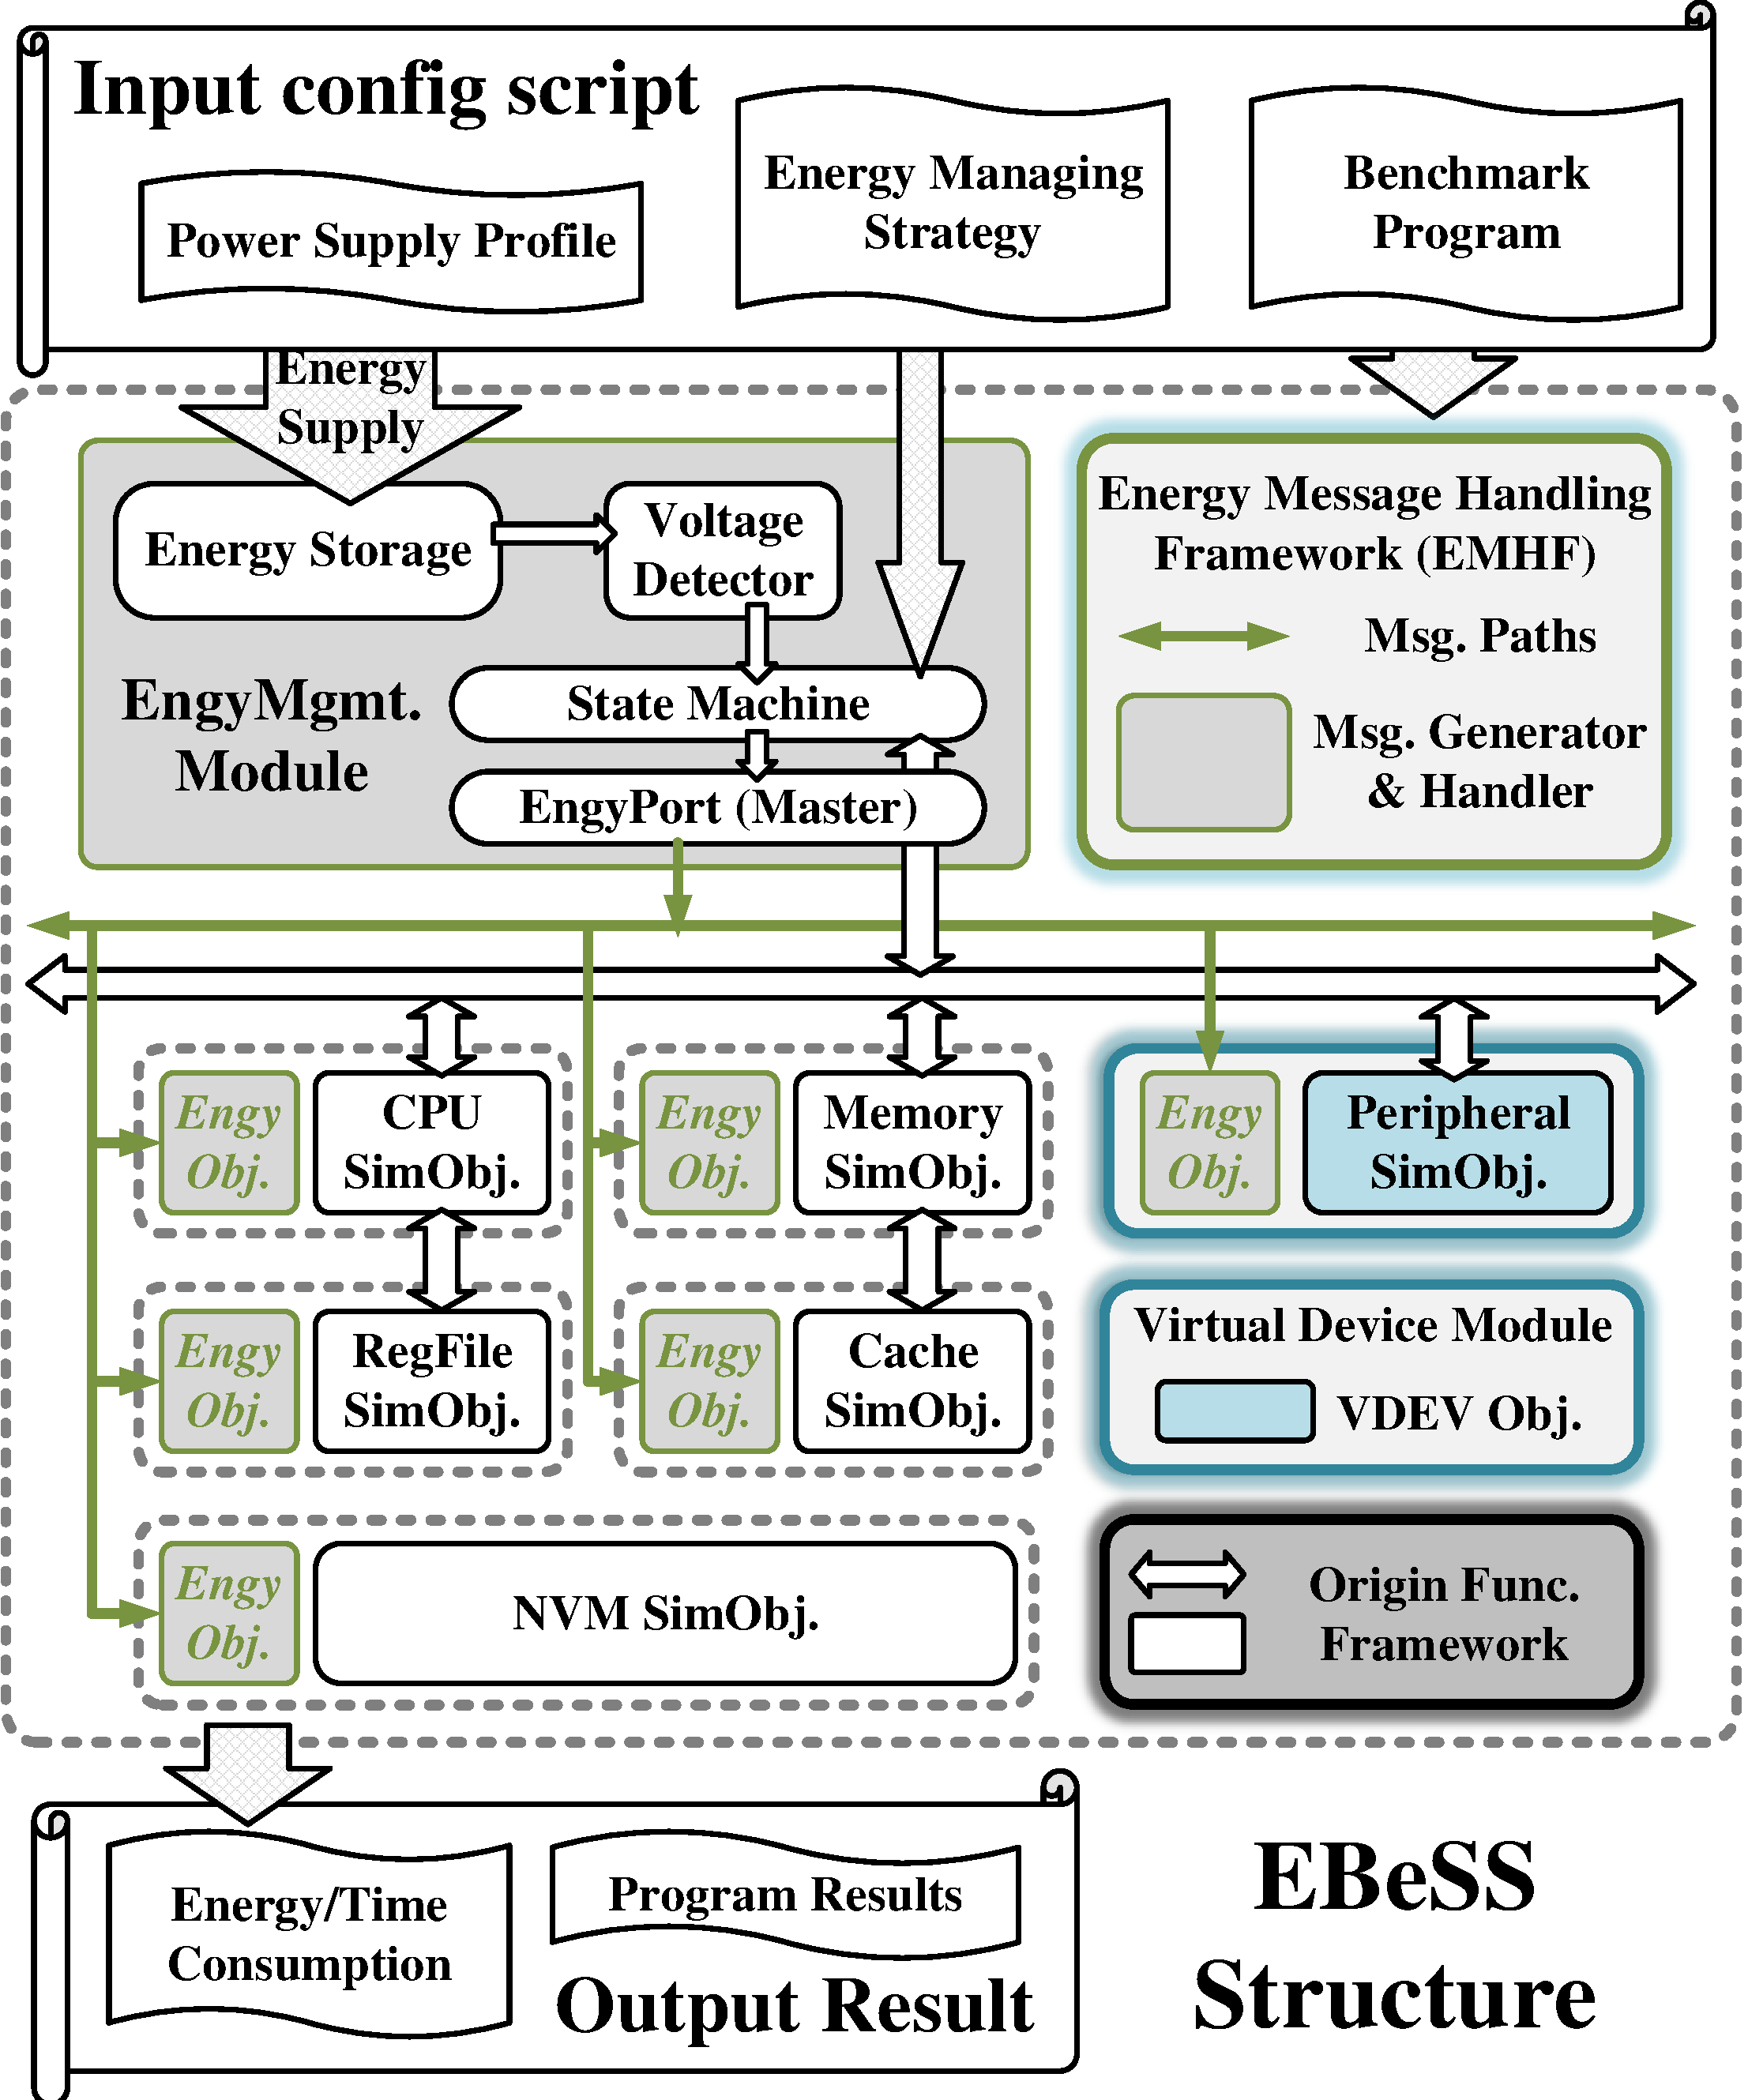
\includegraphics[width=0.5\textwidth]{EBeSS_Structure}
	\vspace{-20pt}
	\caption{Simulator structure of EBeSS. Two new components are added based on original GEM5 architecture. EMHF generates and handles the energy messages according to energy conditions. The virtual device module creates an configurable object that supports the functionary and energy-related behaviors of peripherals.}		\label{fig:techStructure}
\end{figure}

%
To fill the blank of lacking peripheral supports, EBeSS adopts a new simulation object, \emph{virtual device}, which defines the connections and functionary behaviors of various peripherals, as shown in Fig.~\ref{fig:techStructure}.
Virtual device is a configurable, pluggable module connected the system bus, which can be accessed by processor module via virtual addresses. 
Virtual device supports the fundamental operations of a peripheral, including the peripheral register read/write, initialization, activation and interrupts.
Details of the virtual device module is discussed in Sec.~\ref{sec:tech-vdev}.

%
EMHF provides a message-based energy managing framework to support configurable energy managing strategies, as shown in Fig.~\ref{fig:techStructure}.
EMHF contains three components, energy management module (EMM), energy ports and energy objects. 
EMM contains a state machine to generate the state conversion according to user's energy managing strategy. 
Energy ports define the energy message transmission rules and manage the interconnections between EMM and other hardware components.
For each hardware component, EMHF reconstructs it with a new energy-related object, energy object (EnergyObject) allowing energy behaviors defined by energy management strategies as a reaction to energy condition changes.
Details of the energy message handling framework is discussed in Sec.~\ref{sec:tech-EMHF}.


\subsection{Peripheral Support: Virtual Device}	\label{sec:tech-vdev}
%
Although GEM5 provides powerful simulation ability to estimate the functionalities of processor and memories, supports are still vacant for various peripherals, such as sensors and radio transmitter, which play indispensable roles in energy harvesting systems.
To support the peripherals, this subsection first gives a general model of a peripheral and then introduces the proposed hardware component, virtual device.

\textbf{Peripheral Modeling\ \ }
%
Fig.~\ref{} shows a general peripheral structure and its working flow.
Most digital peripherals contain a digital part to connect to the system bus and a analog part to contact with the environment.
The digital part contains a register file to store the command, execution status and data.
The processor accesses the peripheral by writing commands to the \emph{cmd\_reg} and read/write the \emph{data\_reg}.
When the bits in \emph{cmd\_reg} changes, the peripheral triggers an operation, such as initialization and execution.
A peripheral needs to be initialized to ready state before executing a task.
When the task is completed, the peripheral will trigger an interrupt to inform the processor.

\textbf{Virtual Device Object\ \ }
EBeSS proposes a configurable virtual device object defining the peripheral behaviors and the interconnections between peripherals and the processor.
Virtual device is a memory-like module that the processor can make a request by accessing the address of virtual device. 
Considering that most of the energy harvesting systems are light-weighted and lack of operating system supports to automatic allocate address spaces for virtual devices.
EBeSS allows virtual devices to register virtual addresses in the configuration file.
When the processor accesses a registered virtual address, the system will forward this access to the physical address of the related virtual device.
The address of virtual devices consists of a control byte and a maximum 511B internal memory space bytes as data bytes, as shown in Fig.~\ref{fig:VirtualDeviceAddress}.
In the control byte, four bits are used to control the executing status of peripherals.
\emph{addr1} is a configurable \emph{init} bit to trigger the initialization operation.
\emph{addr2} is a read-only \emph{ready} bit representing whether a device is initialized.
\emph{addr5} is a read-only \emph{complete} bit and will be set and trigger an interrupt to the processor, when a virtual device operation is finished.
\emph{addr5} is a read-only \emph{busy} bit representing whether the device is during execution and is not accessible if the bit is set.
\emph{addr7} is a configurable bit set by CPU to make a request to a virtual device.

Fig.~\ref{} shows an example of temperature sensor. 


\begin{figure}[!htpb]
	\centering
	\vspace{-5pt}
	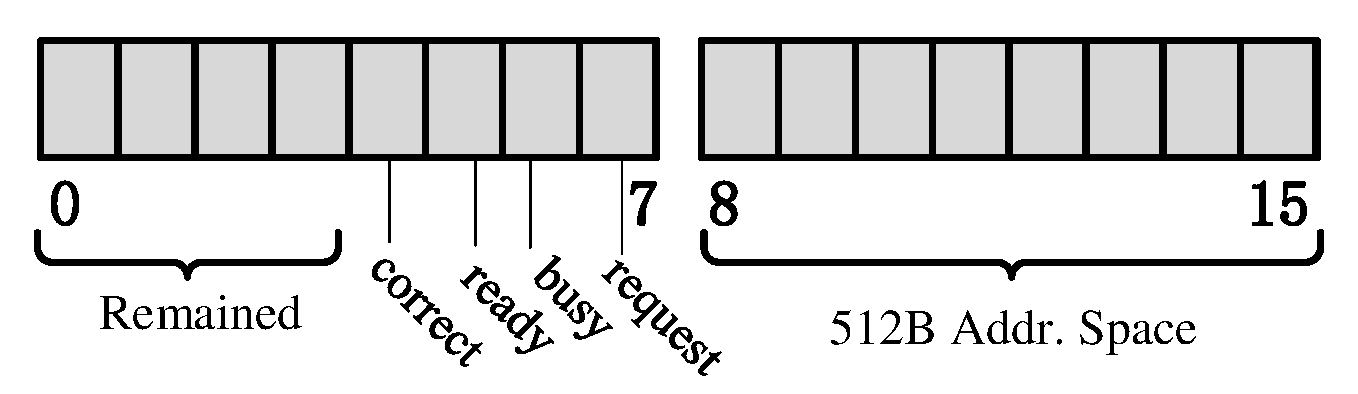
\includegraphics[width=0.4\textwidth]{VirtualDeviceAddress}
	\vspace{-5pt}
	\caption{The bit-level explanation of virtual device address definition.}	\label{fig:VirtualDeviceAddress}
\end{figure}

\subsection{Energy Message Handling Framework (EMHF)}	\label{sec:tech-EMHF}
% Overview
EMHF is a message-based event handling framework to support the energy managing strategies in a self-powered system.
The framework consists of three components: the informer, the connector and the reactor, as shown in Fig.~\ref{fig:EngyMsgFrameworkStructure}. 
With these components, EMHF realize the functionality of energy harvesting, monitoring and all the detailed energy-related behaviors of each hardware component according to energy managing strategies.

\begin{figure}[!htpb]
	\centering
	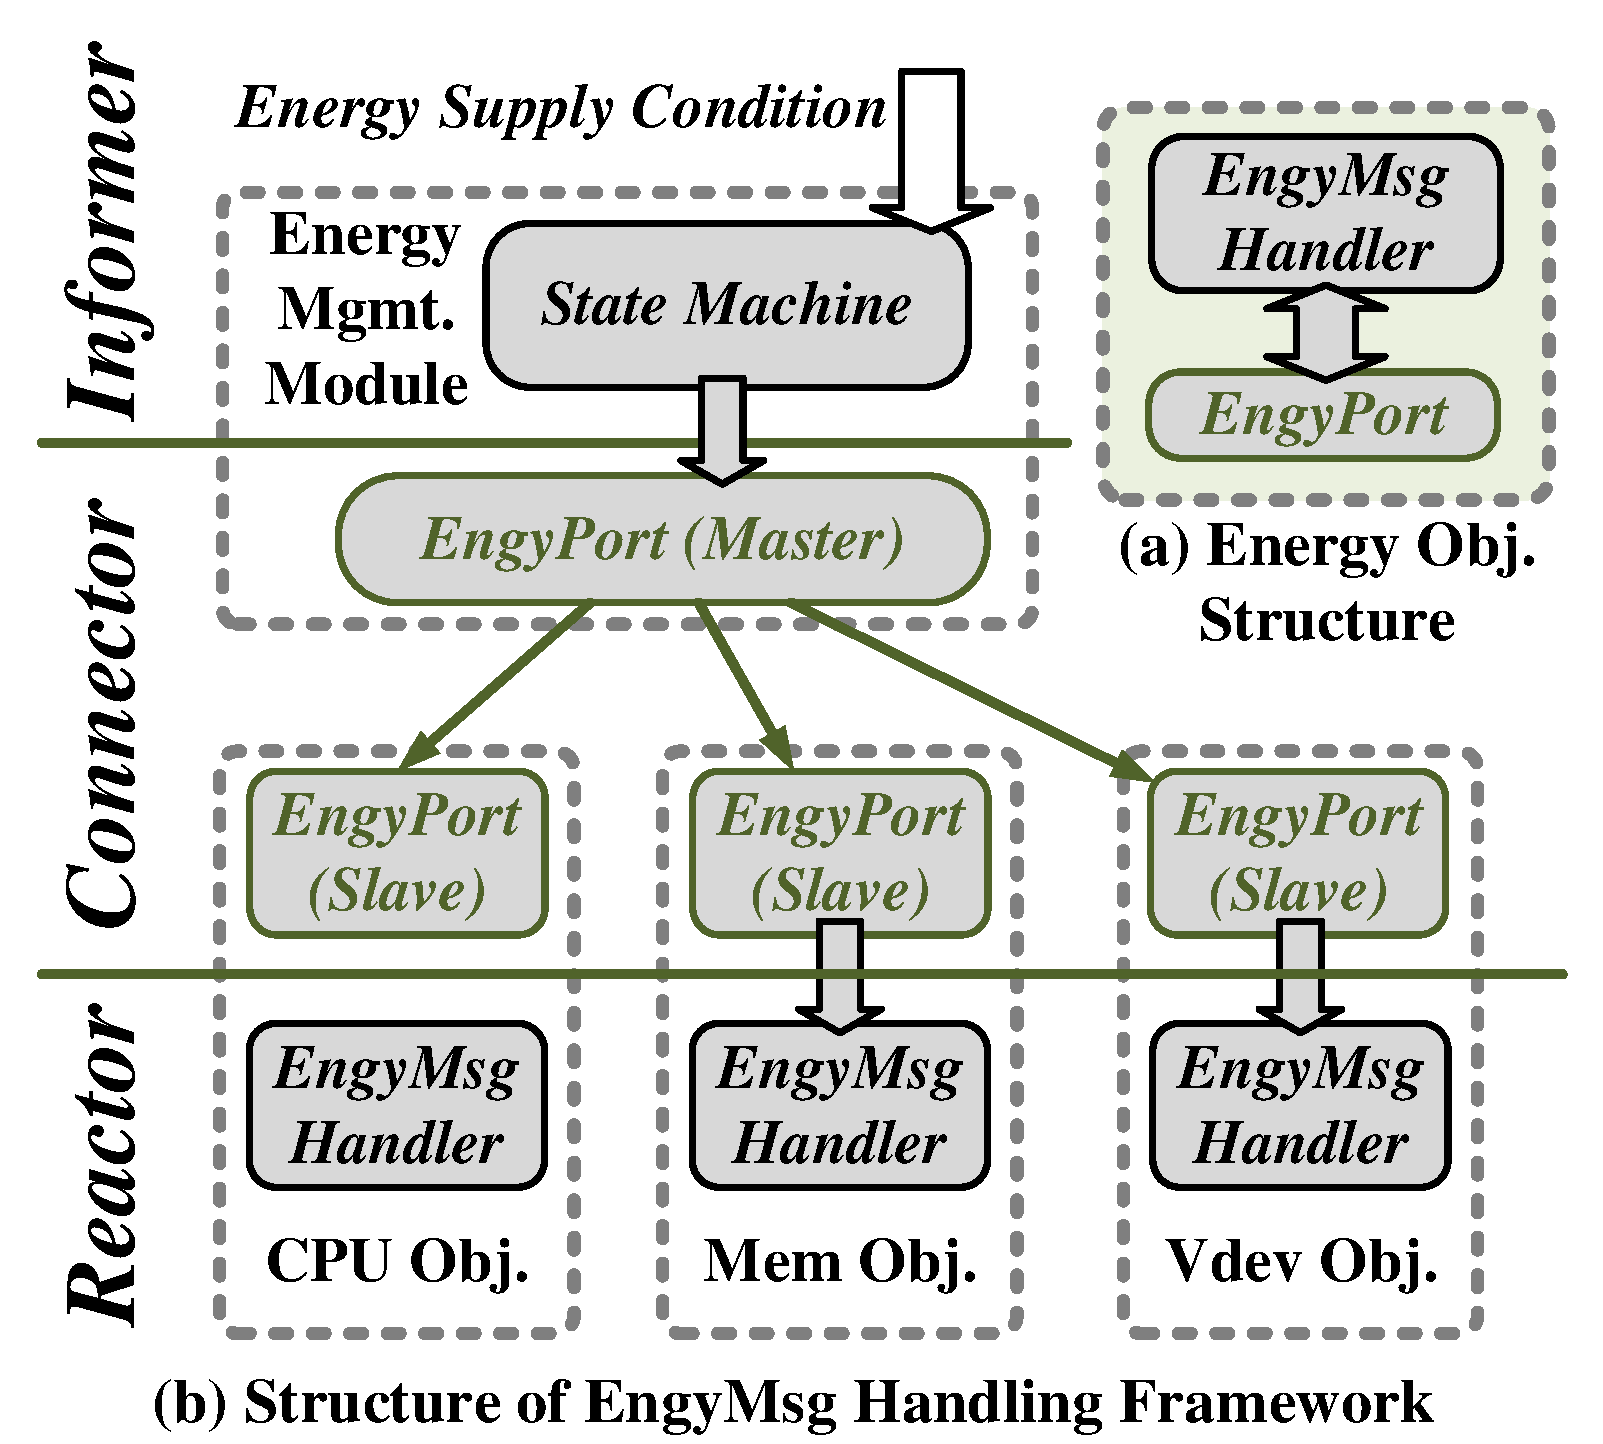
\includegraphics[width=0.45\textwidth]{EngyMsgFrameworkStructure}
	\vspace{-5pt}
	\caption{Structure of the energy message handling framework. The framework contains three components, the informer, the connector and the reactor.}		\label{fig:EngyMsgFrameworkStructure}
	%\vspace{-15pt}
\end{figure}

\textbf{Informer: Energy Management Module.\ \ }
% EMM
In the energy message handling framework, an energy management module (EMM) is developed to monitor energy changes and broadcast state conversion messages according to a user-defined energy managing strategy.
EMM consists of a energy storage, a harvester, a consumer and a state machine, as shown in Fig.~\ref{fig:EnergyManagementModule}. 
During each time tick, the energy harvester collects the income energy from an energy profile and consumer will collect energy consumptions from all the other hardware modules. 
These energy changes are committed to the energy storage (capacitors). 
The state machine is configurable to realize and explore the optimal design of the user-defined energy managing strategies. 
When the supply voltage in the storage reaches certain thresholds, EMM determines state conversion messages according to the state machine and broadcast to the entire system.

\begin{figure}[!htpb]
	\centering
	\vspace{-5pt}
	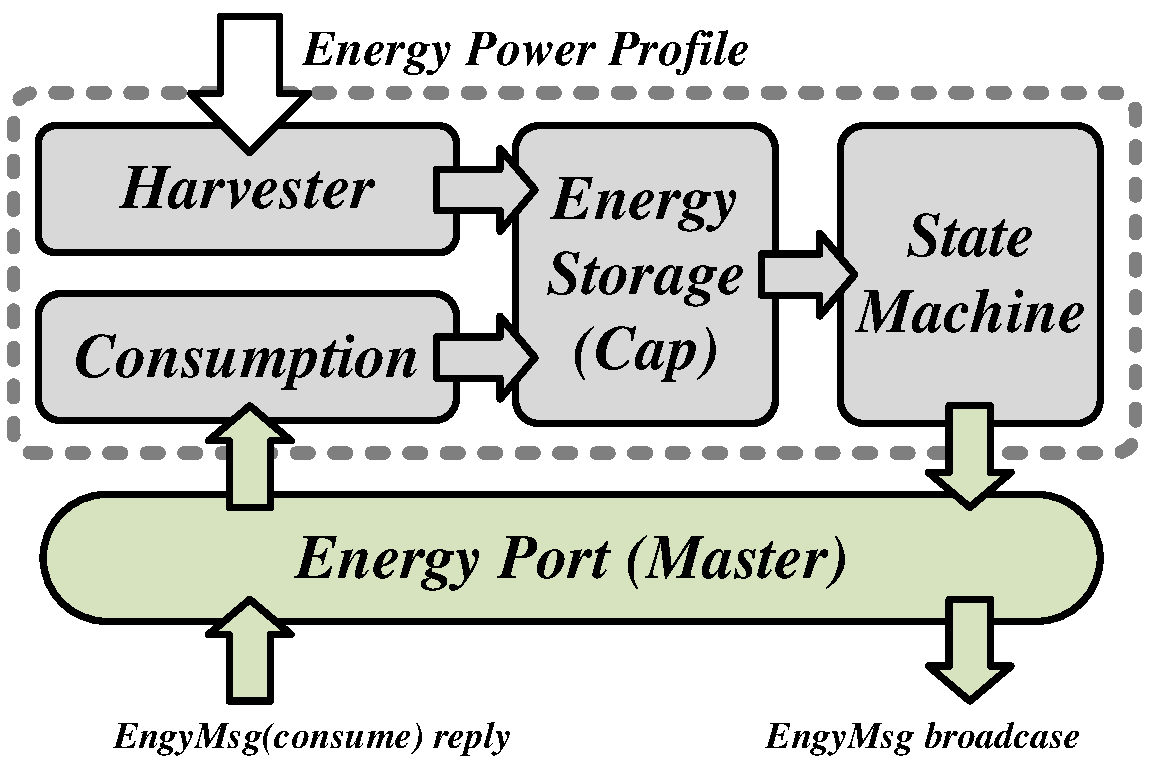
\includegraphics[width=0.35\textwidth]{EnergyManagementModule}
	\vspace{-10pt}
	\caption{The Structure and work flow of the energy Management Module.}		\label{fig:EnergyManagementModule}
\end{figure}

\textbf{Reactor: Energy Object \& Energy Message Handler.\ \ }
% Energy Reactor
Except for EMM, all the other hardware modules are defined as reactors, including the processor, memory and virtual devices.
In GEM5, the native simulation object for these module supports only the functionary behaviors such as computing and memory accessing operations.
To support the energy-related behaviors, EBeSS extend an energy object for each hardware module.
An energy object contain an energy message handler, an consumer and is connected to in EMHF framework via energy ports (introduced later), as shown in Fig.~\ref{fig:EngyMsgFrameworkStructure} (b). 
The energy message handler is a programmable module to realize the detailed reactions defined in an energy managing strategy.
According to developers' needs, the handler will adjust the run-time states and parameters, such as reaction delay, consumption, frequency and register data, to reply the upcoming energy messages.
The consumer is used to manage all the run-time energy consumptions, including execution consumption and leakages.
Every tick or after a message reaction, the consumer should reply its energy consumption in a specific energy consuming message format to EMM to commit the energy costs.
In future, EBeSS will open more authorities that the reactor replying more kinds of energy messages under the premise of system robustness.

\textbf{Connector: The Energy Port.\ \ }
% Energy Port
Energy Ports are interfaces that construct connections and exchange energy messages within EMM and energy objects. 
There are two types of energy ports: master port and slave port.
Master ports are connected to multiple slave ports and maintain a list of its slaves during simulation.
In EBeSS, master port is adopted in EMM module as global energy message informer to actively broadcast energy messages in the entire system.
Slave ports are can only track its unique master.
In EBeSS, all the reactors (hardware modules) are connected to slave ports which is used to receive upcoming energy message and reply consumptions.
Note that, master ports can only connect to slave ports, and vice versa.
All the connections are established by users determining master for each slave port in the configuration profile. 
Currently, only one master port is alternative in EBeSS, hence, all the slave ports have to be connected to EMM.

